% -*- TeX -*-
\documentclass{beamer}

\usepackage{amsmath}
\usepackage{tikz}

\usetikzlibrary{decorations.pathreplacing}
\usetikzlibrary{fit,matrix}

\title{Crustal Deformation Modeling Tutorial}
\subtitle{Spontaneous Rupture via Fault Friction}
\author{Brad Aagaard \\
  Matthew Knepley \\
  Charles Williams}
\institute{
\includegraphics[scale=0.4]{../../logos/cig_blackfg}}
\date{June 28, 2013}


% ---------------------------------------------------- CUSTOMIZATION
\renewcommand{\thispdfpagelabel}[1]{}
\newcommand{\important}[1]{{\color{red}#1}}
\usetheme{CIG}

\newcommand{\tensor}[1]{\overline{#1}}

% ========================================================= DOCUMENT
\begin{document}

% ------------------------------------------------------------ SLIDE
\maketitle

% ------------------------------------------------------------ SLIDE
\logo{
\includegraphics[height=4.5ex]{../../logos/cig_blackfg}}

% ========================================================== SECTION
\section{Introduction}

% ------------------------------------------------------------ SLIDE
\begin{frame}
  \frametitle{Concepts Covered in this Session}
  \summary{}

  \begin{itemize}
  \item PyLith simulations with spontaneous fault rupture
    \begin{itemize}
    \item Quasi-static simulations
    \item Dynamic simulations
    \end{itemize}
  \item Fault constitutive models
    \begin{itemize}
    \item Static friction
    \item Slip-weakening
    \item Dieterich-Ruina rate-state friction w/ageing law
    \end{itemize}
  \item Nonlinear solver parameters
  \item Absorbing boundaries in dynamic simulations
  \item Time-dependent Dirichlet BC
  \item Initial and time-dependent fault traction perturbations
  \end{itemize}

\end{frame}


% ========================================================== SECTION
\section{Implementation}
\subsection{Governing Equations}

% ------------------------------------------------------------ SLIDE
\begin{frame}[fragile]
  \frametitle{Fault Interface}
  \summary{Fault tractions couple deformation across interface}

  \begin{center}
    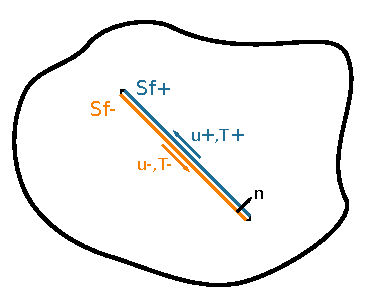
\includegraphics[height=7.0cm]{figs/domaindecomp}
  \end{center}

\end{frame}


% ------------------------------------------------------------ SLIDE
\begin{frame}[fragile]
  \frametitle{Governing Equations}
  \summary{Terms in governing equation associated with fault}

  \begin{itemize}
  \item Tractions on fault surface are analogous to boundary tractions
    \tikz{
      \matrix [matrix of nodes, ampersand replacement=\&] {
      \node {$ \displaystyle \ldots $}; \&
      \node [below delimiter=\}] {$ \displaystyle + \int_{S_T} \vec{\phi} \cdot \vec{T} \, dS$}; \&
      \node [below delimiter=\}] {$ \displaystyle - \int_{S_{f^+}} \vec{\phi} \cdot \vec{l} \, dS$}; \&
      \node [below delimiter=\}] {$ \displaystyle + \int_{S_{f^-}} \vec{\phi} \cdot \vec{l} \, dS$}; \&
      \ldots = 0 \\
      \& \node {Neumann BC}; \& 
      \node {Fault +}; \&
      \node {Fault -}; \& \\
    };
}
  \item Relationship between slip and relative displacement
    \tikz{
      \matrix [matrix of nodes, ampersand replacement=\&] {
        \node {$ \displaystyle \int_{S_f} \vec{\phi} \cdot ($}; \&
        \node [below delimiter=\}] {$\displaystyle\vec{d}$}; \&
        \node {$ \displaystyle - $}; \&
        \node [below delimiter=\}] {$ \displaystyle (\vec{u}_{+} - \vec{u}_{-}) $}; \&
        \node {$ \displaystyle ) dS = 0 $}; \\
        \& Slip \& \& Relative Disp. \& \\
    };
}
  \end{itemize}

\end{frame}


% ------------------------------------------------------------ SLIDE
\begin{frame}
  \frametitle{Governing Equations (cont.)}
  \summary{}

  Express weighting function $\vec{\phi}$, displacement field
  $\vec{u}$, Lagrange multipliers (fault tractions) $\vec{l}$, and
  fault slip $\vec{d}$ as
  linear combinations of basis functions,
  \begin{gather}
    \vec{\phi} = \tensor{N}_m \cdot \vec{a}_m \\
    \vec{u} = \tensor{N}_n \cdot \vec{u}_n \\
    \vec{l} = \tensor{N}_p \cdot \vec{l}_p \\
    \vec{d} = \tensor{N}_p \cdot \vec{d}_p
  \end{gather}

\end{frame}


% ------------------------------------------------------------ SLIDE
\begin{frame}
  \frametitle{Governing Equations (cont.)}
  \summary{}

  \begin{itemize}
  \item Lagrange multiplier (fault traction) terms:
    \begin{equation}
      \ldots 
      - \int_{S_{f^+}} \tensor{N}_m^T \cdot \tensor{N}_p \cdot \vec{l}_p \, dS
      + \int_{S_{f^-}} \tensor{N}_m^T \cdot \tensor{N}_p \cdot \vec{l}_p \, dS
      = \vec{0}
    \end{equation}
  \item Constraint equation
    \begin{equation}
      \int_{S_f} \tensor{N}_p^T \cdot 
      \left( \tensor{N}_p \cdot \vec{d}_p
        - \tensor{N}_{n^+} \cdot \vec{u}_{n^+} 
        + \tensor{N}_{n^-} \cdot \vec{u}_{n^-}
      \right) \, dS = \vec{0}
    \end{equation}
  \end{itemize}

\end{frame}


% ------------------------------------------------------------ SLIDE
\begin{frame}
  \frametitle{Fault Constitutive Model}
  \summary{Fault constitutive model places constraints on Lagrange multipliers}

  \begin{itemize}
  \item Shear components of Lagrange multipliers limited by fault
    constitutive model
    \begin{equation}
      l_\mathit{shear} \leq T_\mathit{friction}
    \end{equation}
  \item Fault friction depends on cohesion, coefficient of friction,
    and normal traction
    \begin{equation}
      T_\mathit{friction} = \left\{ \begin{array}{ll}
          T_\mathit{cohesion} - \mu_\mathit{f} T_\mathit{normal} &
          T_\mathit{normal} \leq 0 \\
          T_\mathit{cohesion} & T_\mathit{normal} > 0
        \end{array} \right.
    \end{equation}
  \item Compression $\Rightarrow$ no interpenetation, opening
    $\Rightarrow$ free surface
    \begin{equation}
      T_\mathit{normal} u_\mathit{normal} = 0 
    \end{equation}
  \end{itemize}
  
\end{frame}


% ------------------------------------------------------------ SLIDE
\begin{frame}
  \frametitle{Solution Algorithm}
  \summary{Solution requires ``friction sensitivity'' solve in
    addition to nonlinear solve}

  \begin{enumerate}
  \item Perform nonlinear iteration assuming no additional slip
  \item Check to see if fault constitutive model is satisfied
  \item If not satisfied, estimate slip required to reduce traction
    \begin{enumerate}
    \item Extract subset of system associated with the fault
      \begin{equation}
        \begin{pmatrix}
          \tensor{K}_{n^+n^+} & 0 & \tensor{L}_p^T  \\
          0 & \tensor{K}_{n^-n^-} & -\tensor{L}_p^T \\
          \tensor{L}_p & -\tensor{L}_p & 0
        \end{pmatrix}
        \begin{pmatrix}
          \vec{u}_{n^+} \\
          \vec{u}_{n^-} \\
          \vec{l}_p \\
        \end{pmatrix}
        =
        \begin{pmatrix}
          \vec{b}_{n^+} \\
          \vec{b}_{n^-} \\
          \vec{b}_p \\
        \end{pmatrix}
      \end{equation}
    \item Perturb Lagrange multipliers to satisfy friction criterion
    \item Inner solve to get slip producing Lagrange multiplier perturbation
      \vspace*{-2mm}
      \begin{gather}
        \tensor{K}_{n^+n^+} \cdot \partial \vec{u}_{n^+} = 
        - \tensor{L}_p^T \cdot \partial \vec{l}_p, \\
        \tensor{K}_{n^-n^-} \cdot \partial \vec{u}_{n^-} =
        \tensor{L}_p^T \cdot \partial \vec{l}_p, \\
        \partial \vec{d}_p =  \partial \vec{u}_{n^+} - \partial \vec{u}_{n^-}.        
      \end{gather}
    \end{enumerate}
  \item Repeat
  \end{enumerate}

\end{frame}


% ------------------------------------------------------------ SLIDE
\begin{frame}
  \frametitle{Friction and Nonlinear Solver Parameters}
  \summary{Solver tolerances are \important{very} important}

  \begin{itemize}
  \item Dynamic (spontaneous rupture) fault has a {\tt
      zero\_tolerance} parameter
  \item Linear solver must converge to tighter tolerance than fault
    {\tt zero\_tolerance} for fault to ``lock''
    \begin{description}
    \item[{\tt ksp\_rtol}] Set to very small value to force absolute
      convergence
    \item[{\tt ksp\_atol}] Must be smaller than fault {\tt
        zero\_tolerance}
    \end{description}
  \item Nonlinear solver tolerance should not be smaller than fault 
    {\tt zero\_tolerance}
    \begin{description}
    \item[{\tt snes\_rtol}] Set to very small value to force absolute
      convergence
    \item[{\tt snes\_atol}] Must be larger than fault {\tt
        zero\_tolerance}
    \end{description}
  \end{itemize}    

\end{frame}


% ------------------------------------------------------------ SLIDE
\begin{frame}[fragile]
  \frametitle{Friction and Nonlinear Solver Parameters}
  \summary{Parameters from a typical example (see examples)}

  \begin{verbatim}
[pylithapp.problem.interfaces.fault]
zero_tolerance = 1.0e-11

[pylithapp.petsc]
# Linear solver tolerances
ksp_rtol = 1.0e-20
ksp_atol = 1.0e-12

# Nonlinear solver tolerances
snes_rtol = 1.0e-20
snes_atol = 1.0e-10

# Set preconditioner for friction sensitivity solve
friction_pc_type = asm
friction_sub_pc_factor_shift_type = nonzero
\end{verbatim}
    
\end{frame}


% ========================================================== SECTION
\subsection{Friction Models}

% ------------------------------------------------------------ SLIDE
\begin{frame}
  \frametitle{Fault Constitutive Models}
  \summary{PyLith contains some of the more popular fault
    constitutive models}

  \begin{tabular}{lp{3in}}
    {\bf\color{green} Static} & Constant coefficient of friction \\
    {\bf\color{green} Slip-Weakening} & Friction decreases with slip to a
    lower limit \\
    {\bf\color{green} Time-Weakening} & Time replaces slip in slip-weakening
    friction model \\
    {\bf\color{green} Rate-State} & Dieterich-Ruina rate-state friction with
    ageing law 
  \end{tabular}
  
  \vfill 
  Some additional, less popular, fault-constitutive models with
  combinations of slip-weakening and time-weakening are available for
  use in the SCEC Dynamic Rupture benchmarks. 
  \vfill

\end{frame}


% ------------------------------------------------------------ SLIDE
\begin{frame}
  \frametitle{Static Friction}
  \summary{Fault has constant coefficient of friction}

  \begin{itemize}
  \item Coefficient of friction
    \begin{equation}
      \mu_f = \mu_\mathit{static}
    \end{equation}
  \item Slip continues once threshold shear traction is reached
  \item No stick-slip behavior
  \item Generally only used in static simulations
  \end{itemize}
  
\end{frame}


% ------------------------------------------------------------ SLIDE
\begin{frame}
  \frametitle{Slip-Weakening Friction}
  \summary{Fault weakens with slip until it reaches a lower limit}

  \begin{equation}
    \mu_f = \left\{ \begin{array}{ll}
        \mu_\mathit{dynamic} + (1 - \frac{D}{D_0})
        (\mu_\mathit{static} -\mu_\mathit{dynamic}) & D \leq D_0 \\
        \mu_\mathit{dynamic} & D > D_0
      \end{array} \right.
  \end{equation}
  \begin{center}
    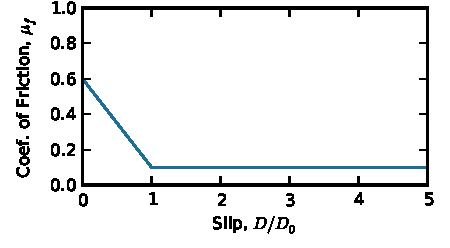
\includegraphics[height=1.65in]{figs/friction_slipweak}
  \end{center}
  
\end{frame}


% ------------------------------------------------------------ SLIDE
\begin{frame}
  \frametitle{Time-Weakening Friction}
  \summary{Fault weakens with time until it reaches a lower limit}
  
  \begin{equation}
    \mu_f = \left\{ \begin{array}{ll}
        \mu_\mathit{dynamic} + (1 - \frac{t}{t_0})
        (\mu_\mathit{static} -\mu_\mathit{dynamic}) & t \leq t_0 \\
        \mu_\mathit{dynamic} & t > t_0
      \end{array} \right.
  \end{equation}
  \begin{center}
    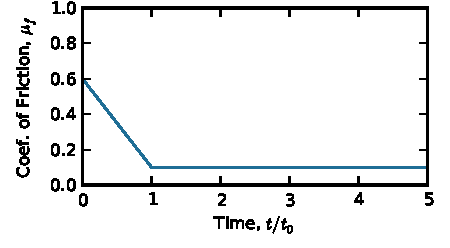
\includegraphics[height=1.65in]{figs/friction_timeweak}
  \end{center}
  
\end{frame}


% ------------------------------------------------------------ SLIDE
\begin{frame}
  \frametitle{Rate-State Friction with Ageing Law}
  \summary{Dieterich-Ruina rate-state friction with ageing evolution law}
  
  \begin{gather}
    \mu_f = \left\{ \begin{array}{ll}
        \mu_0 + a \ln (\frac{V}{V_0}) + b \ln (\frac{V_0 \theta}{L}) & V \ge V_\mathit{linear} \\
        \mu_0 + a \ln (\frac{V_\mathit{linear}}{V_0}) + b \ln
        (\frac{V_0\theta}{L}) - a (1 - \frac{V}{V_\mathit{linear}}) & V
        < V_\mathit{linear}
      \end{array} \right. \\
    \frac{d \theta}{dt} = 1 - \frac{V \theta}{L}
  \end{gather}
  \begin{center}
    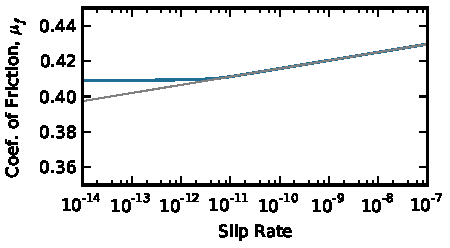
\includegraphics[height=1.65in]{figs/friction_ratestate}
  \end{center}
  
\end{frame}


% ========================================================== SECTION
\subsection{Parameters}

% ------------------------------------------------------------ SLIDE
\begin{frame}
  \frametitle{Spontaneous Rupture Parameters}
  \summary{Overview of principal components}
  
  \begin{tabular}{lp{3in}}
    {\tt\bf\color{green} FaultCohesiveDyn} & Fault object for
    spontaneous rupture \\
    {\tt\bf\color{green}  FrictionModel} & Fault constitutive model \\
    {\tt\bf\color{green}  TractPerturbation} & Prescribed spatial and/or temporal
    variation in fault tractions \\
    {\tt\bf\color{green}  SolverNonlinear} & Quasi-static simulations with
    spontaneous rupture require nonlinear solver
  \end{tabular}
  
\end{frame}


% ------------------------------------------------------------ SLIDE
\begin{frame}[fragile]
  \frametitle{Spontaneous Rupture Parameters}
  \summary{Example of fault parameters in a {\tt .cfg} file}

{\small
\begin{verbatim}
[pylithapp.timedependent.interfaces]
fault = pylith.faults.FaultCohesiveDyn

[pylithapp.timedependent.interfaces.fault]
friction = pylith.friction.StaticFriction
friction.label = Static friction

friction.db_properties = spatialdata.spatialdb.UniformDB
friction.db_properties.label = Static friction
friction.db_properties.values = [friction-coefficient,cohesion]
friction.db_properties.data = [0.6,0.0*Pa]

traction_perturbation = pylith.faults.TractPerturbation
[pylithapp.timedependent.interfaces.fault.traction_perturbation]
db_initial = spatialdata.spatialdb.SimpleDB
db_initial.label = Initial fault tractions
db_initial.iohandler.filename = spatialdb/tractions.spatialdb
\end{verbatim}
}
  
\end{frame}


% ========================================================== SECTION
\section{Examples}
\subsection{examples/3d/hex8}

% ------------------------------------------------------------ SLIDE
\begin{frame}
  \frametitle{Static and Quasi-static Spontaneous Ruptures}
  \summary{Fault slips in response to loading from boundaries}
  
  \vfill
  Files are in {\tt\color{red} examples/3d/hex8}
  \vfill

  \begin{description}
  \item[{\tt Step10}] Static simulation, static friction w/o slip
  \item[{\tt Step11}] Static simulation, static friction w/slip
  \item[{\tt Step12}] Quasi-static simulation, static friction w/slip
  \item[{\tt Step13}] Quasi-static simulation, slip-weakening w/stick-slip
  \item[{\tt Step14}] Quasi-static simulation, rate-state w/stick-slip
  \end{description}
  
  \vfill
  {\tt pylith step10.cfg}
  \vfill

\end{frame}


% ------------------------------------------------------------ SLIDE
\begin{frame}
  \frametitle{{\tt Step11}}
  \summary{Static simulation, static friction w/slip}

  \begin{center}
    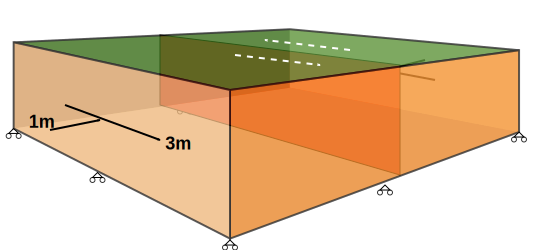
\includegraphics[width=4.0in]{figs/step11_schematic}
  \end{center}
  
\end{frame}


% ------------------------------------------------------------ SLIDE
\begin{frame}
  \frametitle{{\tt Step13}}
  \summary{Quasi-static simulation, slip-weakening w/slip-slip}
  
  \begin{center}
    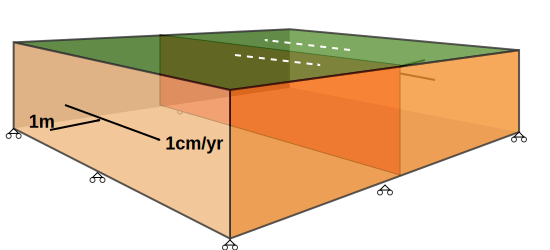
\includegraphics[width=4.0in]{figs/step13_schematic}
  \end{center}
  
\end{frame}


% ========================================================== SECTION
\subsection{examples/bar\_shearwave/quad4}

% ------------------------------------------------------------ SLIDE
\begin{frame}
  \frametitle{Dynamic Spontaneous Rupture}
  \summary{Fault slips in reponse to prescribed tractions}
  
  \vfill
  Files are in {\tt\color{red} examples/bar\_shearwave/quad4}
  \vfill

  \begin{description}
  \item[{\tt spontaneousrup\_staticfriction}] Static friction
  \item[{\tt spontaneousrup\_slipweakening}] Slip-weakening
  \item[{\tt spontaneousrup\_ratestateageing}] Rate-state w/ageing law
  \end{description}
  
  \vfill
  {\tt pylith spontaneousrup.cfg spontaneousrup\_staticfriction.cfg}
  \vfill

\end{frame}


% ------------------------------------------------------------ SLIDE
\begin{frame}
  \frametitle{Prescribed Traction Loads Fault}
  \summary{Dynamic simulation w/initial \& temporal traction perturbation}

  \begin{center}
    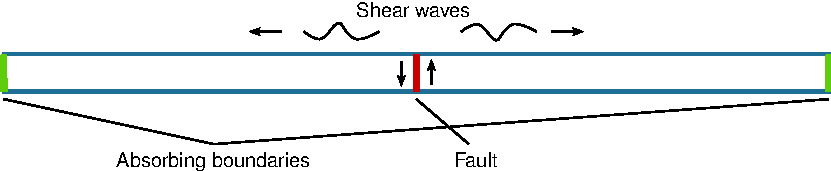
\includegraphics[width=10.0cm]{figs/bar}\\ \vspace*{0.5cm}
    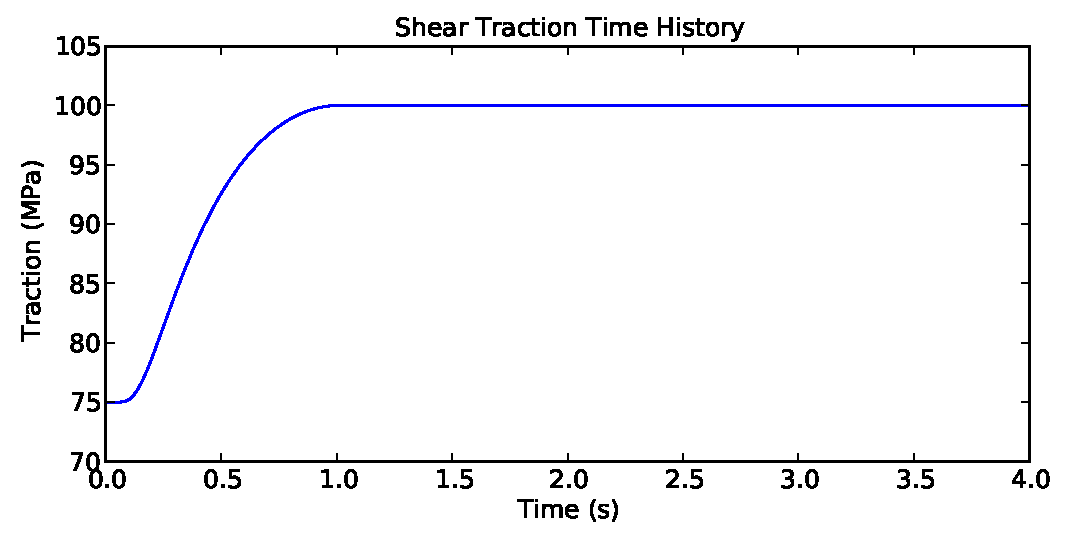
\includegraphics[width=8.0cm]{figs/bar_tractionth}
  \end{center}
  
\end{frame}


% ======================================================================
\end{document}


% End of file
